\documentclass[a4paper,10pt]{article}
\usepackage[top=2cm, bottom=2cm, left=3cm, right=3cm, heightrounded]{geometry}
\usepackage{fancyhdr}
\usepackage{tabularx}
\usepackage{glossaries}
\usepackage[misc]{ifsym}
\pagestyle{fancy}
\usepackage{amsmath}
\usepackage{enumitem}
\setlist{nosep}
\usepackage{mathtools}
\usepackage[]{hyperref}
\usepackage{xcolor}
\hypersetup{
    colorlinks,
    linkcolor={red!50!black},
    citecolor={blue!50!black},
    urlcolor={blue!80!black}
}
\usepackage{todonotes}
\usetikzlibrary{fit,calc,arrows,arrows.meta}
\usepackage{booktabs}
\usepackage[framemethod=tikz,outerlinewidth=0,linewidth=0pt]{mdframed}
\usepackage{amssymb}
%\usepackage{ebgaramond}
%\usepackage[sfdefault,light]{FiraSans}
\usepackage[default]{opensans}
\usetikzlibrary{external}
\tikzexternalize

\newcommand\MAILTO[2]{#1 \Letter\; \href{mailto:#2}{\nolinkurl{#2}}}
\newcommand\MAILTOBREAK[2]{#1 \Letter\; \href{mailto:#2}{\nolinkurl{#2}}}

\author{NCBS Bangalore}
\title{Student Hanbook}
\date{\today}

\begin{document}

\newglossaryentry{tcm} 
{
    name=TCM,
    description={Thesis Committee Meeting}
}

\newglossaryentry{ce} 
{
    name=CE,
    description={Comprehensive Examination}
}


The purpose of this handbook is to outline the procedures for students to receive a degree.
This handbook will be updated annually in August. Any major changes made prior to that
time will be posted to our website with notification to all graduate students by email. The
information in this handbook should be viewed as guidelines and are subject to change
depending on the policies of the Institutes.

\vspace{10cm}

\begin{mdframed}[frametitle=\textsc{Honor Code},backgroundcolor=yellow!20]
Our community operates on a principle of trust. Most research materials are kept
in accessible locations. Research on our campus depends critically on colleagues
being able to trust each other’s data.  Any form of cheating, plagiarism, or
falsification of data is unacceptable and will invite appropriate consequences.
\end{mdframed}

\newpage
\tableofcontents 

\newpage
\section{Academic Calendar}
\label{sec:academic_calendar}

It is the student’s responsibility to ensure they meet all requirements and
deadlines. 

\marginpar{\footnotesize TCM:  Thesis Committee Meeting}
\marginpar{\footnotesize CE: Comprehensive Examination}


\subsection{PhD Calendar}
%\RequirePackage{luatex85}
\documentclass[crop,tikz]{standalone}
\usetikzlibrary{calc,positioning,fit,arrows,arrows.meta}
\usepackage[sfdefault,light]{FiraSans}
\begin{document}

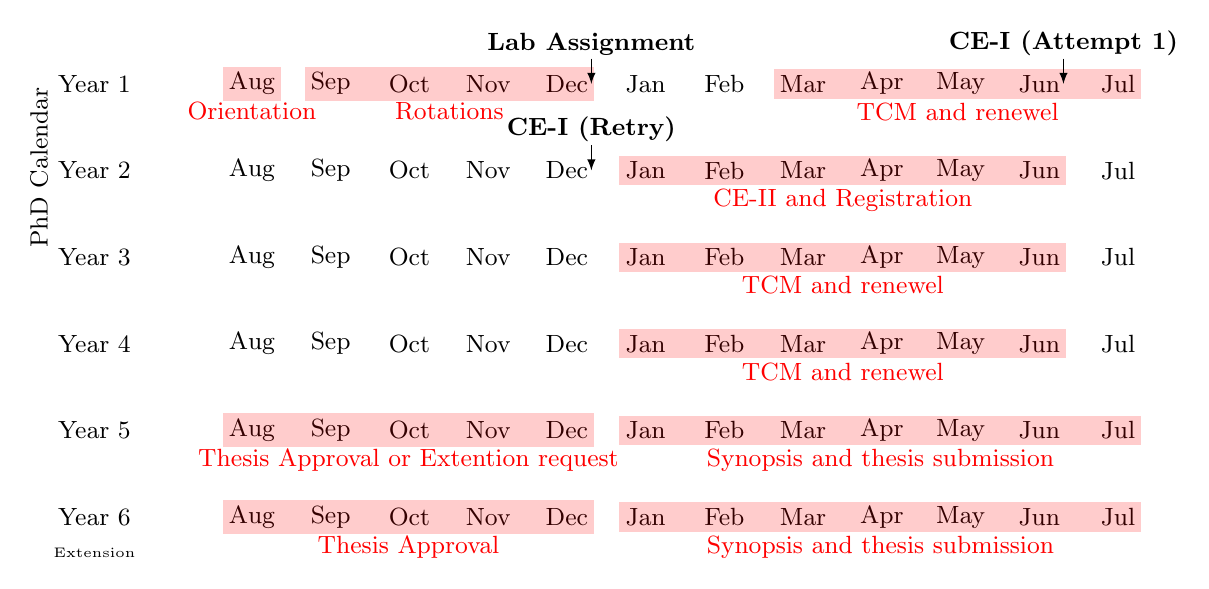
\begin{tikzpicture}[scale=1
    , every node/.style={node distance=2mm,inner sep=1pt}
]
    \small
    \edef\dy{-1.2mm}
    \edef\gap{1.1}
    \foreach \y in {1,2,3,4,5,6}
    {
        \node (year\y) at (-1,-\gap * \y cm) {Year \y};
        \foreach \month[count=\m] in {Aug,Sep,Oct,Nov,Dec,Jan,Feb,Mar,Apr,May,Jun,Jul}
        \node[] (year\y month\m) at (\m,-\gap * \y cm) {{\month}};
    }

    \node[below=of year6]{{\tiny Extension}};
    \node[left=of year1,rotate=90] {PhD Calendar};

    % Orientation.
    \def\cl{red}
    \node[fit=(year1month1),fill=\cl,opacity=0.2] (orientation) {};
    \node[below=of orientation.center] {\textcolor{\cl}{Orientation}};

    % Rotation
    \node[fill=\cl,opacity=0.2,fit= (year1month2) (year1month5) ] (rotations) { };
    \node[below=of rotations.center] {\textcolor{\cl}{Rotations}};

    \node[above=of year1month5.east,yshift=-\dy]  (labassignments) {\bf Lab Assignment};
    \draw[-latex] (labassignments) -- (year1month5.east);

    % TCM
    \node[fill=\cl,opacity=0.2,fit=(year1month8) (year1month12)] (tcm) { };
    \node[below=of tcm.center] {\textcolor{\cl}{TCM and renewel}};

    % CE
    \node[above=of year1month11.east,yshift=-\dy] (ce1) {\bf CE-I (Attempt 1)};
    \draw[-latex] (ce1) -- (year1month11.east);
    
    \node[above=of year2month5.east,yshift=-\dy] (ce2) {\bf CE-I (Retry)};
    \draw[-latex] (ce2) -- (year2month5.east);

    % Registration
    \node[fill=\cl,opacity=0.2,fit=(year2month6) (year2month11)] (reg) { };
    \node[below=of reg.center] 
        {\textcolor{\cl}{CE-II and Registration}};

    % TCM
    \node[fill=\cl,opacity=0.2,fit=(year3month6) (year3month11)] (tcm) { };
    \node[below=of tcm.center] {\textcolor{\cl}{TCM and renewel}};


    \node[fill=\cl,opacity=0.2,fit=(year4month6) (year4month11)] (tcm) { };
    \node[below=of tcm.center] {\textcolor{\cl}{TCM and renewel}};

    % Thesis 
    \node[fill=\cl,opacity=0.2,fit=(year5month1) (year5month5)] (thesis) { };
    \node[below=of thesis.center] 
        {\textcolor{\cl}{Thesis Approval or Extention request}};

    \node[fill=\cl,opacity=0.2,fit=(year5month6) (year5month12)] (thesis1) { };
    \node[below=of thesis1.center] 
        {\textcolor{\cl}{Synopsis and thesis submission}};

    % Thesis 
    \node[fill=\cl,opacity=0.2,fit=(year6month1) (year6month5)] (thesis) { };
    \node[below=of thesis.center] 
        {\textcolor{\cl}{Thesis Approval}};

    \node[fill=\cl,opacity=0.2,fit=(year6month6) (year6month12)] (thesis1) { };
    \node[below=of thesis1.center] 
        {\textcolor{\cl}{Synopsis and thesis submission}};




    


\end{tikzpicture}    

\end{document}


\subsection{Int-PhD Calendar}
%\RequirePackage{luatex85}
\documentclass[crop,tikz]{standalone}
\usetikzlibrary{calc,positioning,fit,arrows,arrows.meta}
\usepackage[sfdefault,light]{FiraSans}
\begin{document}

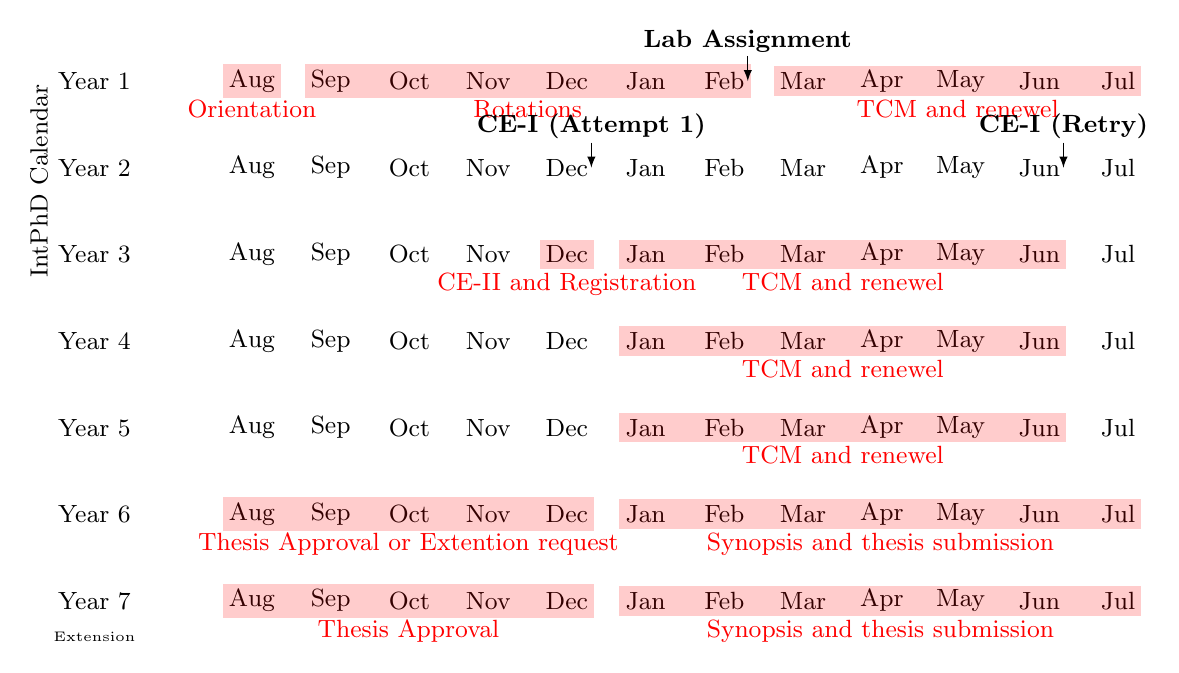
\begin{tikzpicture}[scale=1
    , every node/.style={node distance=2mm,inner sep=1pt}
]
    \small
    \edef\dy{-1.2mm}
    \edef\gap{1.1}
    \foreach \y in {1,2,3,4,5,6,7}
    {
        \node (year\y) at (-1,-\gap * \y cm) {Year \y};
        \foreach \month[count=\m] in {Aug,Sep,Oct,Nov,Dec,Jan,Feb,Mar,Apr,May,Jun,Jul}
        \node[] (year\y month\m) at (\m,-\gap * \y cm) {{\month}};
    }

    \node[below=of year7]{{\tiny Extension}};
    \node[left=of year1,rotate=90] {IntPhD Calendar};

    % Orientation.
    \def\cl{red}
    \node[fit=(year1month1),fill=\cl,opacity=0.2] (orientation) {};
    \node[below=of orientation.center] {\textcolor{\cl}{Orientation}};

    % Rotation 1 and 2.
    \node[fill=\cl,opacity=0.2,fit= (year1month2) (year1month7) ] (rotations) { };
    \node[below=of rotations.center] {\textcolor{\cl}{Rotations}};

    \node[above=of year1month7.east,yshift=-\dy]  (labassignments) {\bf Lab Assignment};
    \draw[-latex] (labassignments) -- (year1month7.east);

    % TCM
    \node[fill=\cl,opacity=0.2,fit=(year1month8) (year1month12)] (tcm) { };
    \node[below=of tcm.center] {\textcolor{\cl}{TCM and renewel}};

    % CE
    \node[above=of year2month5.east,yshift=-\dy] (ce1) {\bf CE-I (Attempt 1)};
    \draw[-latex] (ce1) -- (year2month5.east);
    
    \node[above=of year2month11.east,yshift=-\dy] (ce2) {\bf CE-I (Retry)};
    \draw[-latex] (ce2) -- (year2month11.east);

    % Registration
    \node[fill=\cl,opacity=0.2,fit=(year3month5)] (reg) { };
    \node[below=of reg.center] 
        {\textcolor{\cl}{CE-II and Registration}};

    % TCM
    \node[fill=\cl,opacity=0.2,fit=(year3month6) (year3month11)] (tcm) { };
    \node[below=of tcm.center] {\textcolor{\cl}{TCM and renewel}};


    \node[fill=\cl,opacity=0.2,fit=(year4month6) (year4month11)] (tcm) { };
    \node[below=of tcm.center] {\textcolor{\cl}{TCM and renewel}};

    \node[fill=\cl,opacity=0.2,fit=(year5month6) (year5month11)] (tcm) { };
    \node[below=of tcm.center] {\textcolor{\cl}{TCM and renewel}};


    % Thesis 
    \node[fill=\cl,opacity=0.2,fit=(year6month1) (year6month5)] (thesis) { };
    \node[below=of thesis.center] 
        {\textcolor{\cl}{Thesis Approval or Extention request}};

    \node[fill=\cl,opacity=0.2,fit=(year6month6) (year6month12)] (thesis1) { };
    \node[below=of thesis1.center] 
        {\textcolor{\cl}{Synopsis and thesis submission}};

    % Thesis 
    \node[fill=\cl,opacity=0.2,fit=(year7month1) (year7month5)] (thesis) { };
    \node[below=of thesis.center] 
        {\textcolor{\cl}{Thesis Approval}};

    \node[fill=\cl,opacity=0.2,fit=(year7month6) (year7month12)] (thesis1) { };
    \node[below=of thesis1.center] 
        {\textcolor{\cl}{Synopsis and thesis submission}};

\end{tikzpicture}    

\end{document}


\subsection{MSc Calendar}
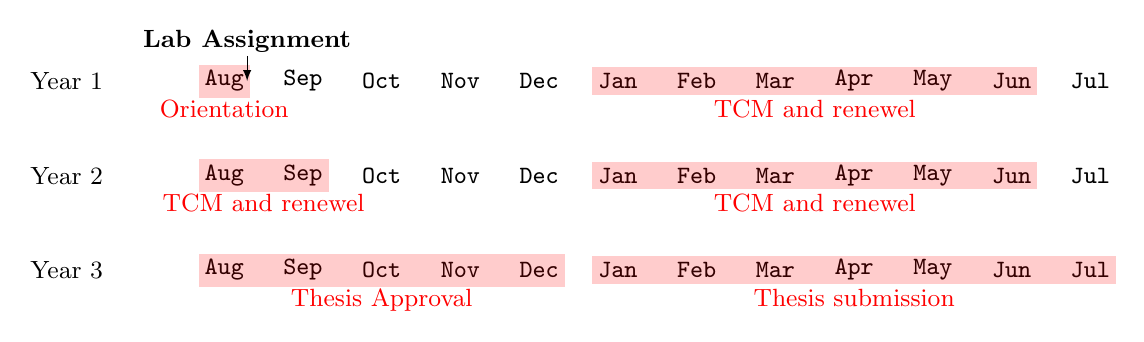
\begin{tikzpicture}[scale=1
    , every node/.style={node distance=2mm,inner sep=1pt}
]
    \small
    \edef\dy{-1.2mm}
    \edef\gap{1.2}
    \foreach \y in {1,2,3}
    {
        \node (year\y) at (-1,-\gap * \y cm) {Year \y};
        \foreach \month[count=\m] in {Aug,Sep,Oct,Nov,Dec,Jan,Feb,Mar,Apr,May,Jun,Jul}
        \node[] (year\y month\m) at (\m,-\gap * \y cm) {\texttt{\month}};
    }

    % Orientation.
    \def\cl{red}
    \node[fit=(year1month1),fill=\cl,opacity=0.2] (orientation) {};
    \node[below=of orientation.center] {\textcolor{\cl}{Orientation}};

    \node[above=of year1month1.east,yshift=-\dy]  (labassignments) {\bf Lab Assignment};
    \draw[-latex] (labassignments) -- (year1month1.east);

    % TCM
    \node[fill=\cl,opacity=0.2,fit=(year1month6) (year1month11)] (tcm) { };
    \node[below=of tcm.center] {\textcolor{\cl}{TCM and renewel}};

    \node[fill=\cl,opacity=0.2,fit=(year2month1) (year2month2)] (tcm) { };
    \node[below=of tcm.center] {\textcolor{\cl}{TCM and renewel}};

    \node[fill=\cl,opacity=0.2,fit=(year2month6) (year2month11)] (tcm) { };
    \node[below=of tcm.center] {\textcolor{\cl}{TCM and renewel}};

    % Thesis 
    \node[fill=\cl,opacity=0.2,fit=(year3month1) (year3month5)] (thesis) { };
    \node[below=of thesis.center] 
        {\textcolor{\cl}{Thesis Approval}};

    \node[fill=\cl,opacity=0.2,fit=(year3month6) (year3month12)] (thesis1) { };
    \node[below=of thesis1.center] 
        {\textcolor{\cl}{Thesis submission}};

\end{tikzpicture}    



\newpage
\section{Where to go for help}

\subsection{Academic Office} 
All student academic matters, including scheduling
Annual Work Seminars, submission of Thesis Advisory Committee reports, course
transcripts, interactions with MU or TIFR, and thesis submission.

\begin{itemize}
    \item \MAILTO{Academic Office}{acadoffice@ncbs.res.in} 
    \item \MAILTO{Ms. K. S. Vishalakshi}{ksvishal@ncbs.res.in}
\end{itemize}

\subsection{Establishment and Administrative Office}
Joining formalities, extramural fellowships, interface with outside agencies.

\begin{itemize}
    \item \MAILTO{Admin Help}{adminhelp@ncbs.res.in}
    \item \MAILTO{Mr. Ashok Rao}{ashok@ncbs.res.in}
    \item \MAILTO{Mr. A. Ramachandra}{anramachandra@instem.res.in}
\end{itemize}

\subsection{Miscellenous}

\begin{tabularx}{\textwidth}{l X X}
    \toprule
    Service & Supervisor & Notes \\
    \midrule
    Main reception & \MAILTOBREAK{Anand Kumar}{reception@ncbs.res.in} & Any general enquiry \\
    Air conditioning & \MAILTOBREAK{HS Venkataramana}{achelp@ncbs.res.in} & AC issues \\
    Animal care facility & \MAILTOBREAK{Dr. Mohan}{mohan@ncbs.res.in} & Aninal
        procedures. Note that its not a helpdesk queue.  \\
    Civil and Interiors & \MAILTOBREAK{Mr. H.M. Basavaraja, Ms.
    Savitha}{civilint@ncbs.res.in} & Civil engineering, plumbing, paints,
        furniture and interiors, gardening \\
    Computer services & \MAILTOBREAK{Mr. Prasanta Baruah}{ithelp@ncbs.res.in} & 
        Computer hardware and software, internet services \\
    Electricals & \MAILTOBREAK{ Mr. Suresh Kumar}{elechelp@ncbs.res.in} & 
            Electrical issues, wiring, lighting \\
    Electronic Workshop & \MAILTOBREAK{Mr.  Dorababu}{elecworkshop@ncbs.res.in} & 
        Electronic components, PCB \\
    Hostel and Canteen & \MAILTOBREAK{Mr. Shaju Varghese}{hospitality@ncbs.res.in} & 
        Canteen, guest house, hostel, lab cleaning, bathrooms \\
    Instrumentation & \MAILTOBREAK{Mr. P.C. Gautam}{instrumentation@ncbs.res.in} &
        Lab equipment, UPSs, telecom issues, projectors, videoconferencing \\
    Labkitchen & \MAILTOBREAK{ }{labkitchen@ncbs.res.in} & Gas cylinders, media, glassware \\
    Library & \MAILTOBREAK{Mr. A.D. Chinchure}{library@ncbs.res.in} &
        library Books, journals, online resources. Note that its not a helpdesk
        queue \\
    Room booking & \MAILTOBREAK{ }{bookmyvenue@ncbs.res.in} & All room bookings \\
    Transport & \MAILTOBREAK{}{transport@ncbs.res.in} & Local transport \\
    \bottomrule
\end{tabularx}


\newpage
\section{Programmes of study}

Our programmes target students who intend to pursue research careers in interdisciplinary
areas within or outside academia. Our main goal is to provide you with a strong technical
background and the capacity for analytical thinking. Your experience here will prepare you
to be academic leaders with a competence to define and solve new kinds of problems for the
advancement of science and society.

\subsection{PhD Programme}
NCBS and inStem offer a graduate programme leading to the award of a
PhD degree for students holding a Masters degree in a basic science, or a Bachelors degree
in any applied science. The standard tenure is 5 years. Students from NCBS are registered at
TIFR Mumbai, and those from inStem at Manipal University.

\subsection{Integrated MSc-PhD Programme}
NCBS offers a graduate programme leading to the
award of a PhD degree for students holding a Bachelors degree in any basic or applied
science. Students from 4-year Bachelors programmes can opt to be considered either for the
Int-PhD or the PhD stream during the application process. The standard tenure is 6 years.
Students are registered at TIFR Mumbai.

\subsection{MSc-by-Research Programme}
Candidates applying for the Int-PhD programme may
sometimes be offered a position in the NCBS MSc-by-Research programme. Selected
students must identify a suitable host laboratory and be funded on extramural grants. The
standard tenure is 3 years. Students are registered at TIFR Mumbai.

\subsection{MSc in Wildlife and Conservation} NCBS, the Centre for Wildlife
Studies (CWS), and the Wildlife Conservation Society (WCS) jointly run the MSc
in Wildlife and Conservation programme. This two-year programme is organized
into three semesters of course work, and a final semester of field research and
thesis preparation. Students are registered at TIFR Mumbai. \footnote{
    \textbf{TIFR Academic Structure} The Tata Institute of Fundamental Research
    has been deemed a University. The Academic Council of the TIFR exercises
    oversight over the functioning of the University, setting policy, initiating
    new programmes and approving the award of degrees recommended by the Subject
    Boards. The AC is chaired by the Director, TIFR and among its external
    members are three appointed by the UGC. TIFR conducts Academic programmes
    leading to PhD and MSc degrees. These programmes are supervised by Subject
    Boards for Biology, Chemistry, Computer Science, Mathematics, Physics, and
    Science Education. The Biology Subject Board has members from DBS, Mumbai
    and from NCBS, Bangalore with Professor Upinder Bhalla as the convenor. The
    Board Guidelines specify coursework requirements and evaluation norms for
    students and also oversees the thesis examination process. The Board chooses
    examiners for PhD and MSc theses and authorizes a viva voce examination when
    all concerns are addressed. Once the student passes the examination, the
    Board recommends award of the relevant degree.
}


\section{Student Categories}

\subsection{PhD and Int-PhD Research Scholars}

Candidates for the PhD and Int-PhD programmes are invited to apply in response
to advertisements appearing in national newspapers in August every year.
Candidates short-listed on the basis of their written test performance, academic
record, statement of purpose, and letters of evaluation finally selected through
an on-campus interview conducted each summer. Research Scholars are supported
from core NCBS or inStem institutional funds throughout their standard tenure.
We encourage Research Scholars to apply for external fellowships. If the
fellowship pays less than the scholarship amount, the institute will pay the
difference.  

\subsection{MSc-by-Research Students}
Each year a set of Int-PhD candidates are
offered a position in the MSc-by-Research programme. MSc students must identify
and directly join a host laboratory at NCBS. They may be supported through CSIR,
ICMR or DBT fellowships, or through an extramural grant from their host
Principal Investigators. Admission and continuation in both situations is
contingent on association with the PI’s laboratory.  Contingency grants are not
provided for students in this programme.

\subsection{MSc in Wildlife and Conservation}
Students selected to this programme are supported through core programme funds.
These students are not affiliated with any laboratory; instead, their training,
fieldwork, and research are coordinated by the Program Directors. 

\subsection{Transfer students from other TIFR Centres}
Physics, Chemistry, Biology or Computer
Science students already enrolled in the PhD programmes at other TIFR campuses
may conduct their research work at NCBS under the guidance of an NCBS faculty
member. Such students can transfer within TIFR to NCBS and will have to meet the
academic requirements of NCBS. Similarly, NCBS students may work with faculty
members at other TIFR Centres.  These transfers should be coordinated with Head
Academics, and with the appropriate Subject Board Convenors. 

\subsection{Externally registered PhD students}
A small number of talented candidates with fellowships
from CSIR or other funding agencies may utilize these fellowships to work in our
laboratories and if recommended by their faculty mentor, register at outside
institutions, which recognize our faculty as guides.  Externally funded Junior
Research Fellows: Students with fellowships from CSIR/UGC/ICMR/DBT/DST or other
agencies may utilize these fellowships to work as JRFs at NCBS and inStem.
Candidates interested in JRF positions must contact host laboratories directly.
Faculty members may recommend exceptional JRFs or other candidates to be
interviewed for entry into the graduate programme during the regular NCBS and
inStem interviews conducted each summer. 

\paragraph{Regulations and fees} All students must follow the rules and
regulations applicable to Research Scholars and will enjoy the same campus
privileges. A tuition grant is awarded to all students in the PhD or Int-PhD
programme to meet the requirements of tuition fees at TIFR or MU. Fees for
externally-registered PhD students on grants and students in the MScby-Research
programme are covered by extramural funds available to the student or the PI.
	

\section{PhD and Integrated PhD} 

\subsection{Degree Awarding Institutions}
Students enrolled in the PhD and Int-PhD programmes at NCBS are awarded degrees
by TIFR, Mumbai. Students enrolled in the PhD programme at inStem are awarded
the degree by Manipal University.  

\subsection{Orientation and Rotations}
New students must
arrive on campus by August 1 each year and must attend an Orientation Programme
which runs for three weeks. In this programme, students meet with faculty
members and their research groups. They are also informed about Research,
Technical and Administrative services on campus. At the end of the Orientation
Programme, and at the end of each rotation, students must select a host
laboratory for their next rotation. Rotation slots must be mutually agreed by
students and their hosts. Once a decision of host laboratory is made, students
should request the host to send a confirmation email to the Academic Office
(acadoffice@ncbs.res.in). It is the responsibility of the student to ensure that
this email is sent by the host PI on time, at the latest by the Thursday prior
to the start of the rotation. Head Academics might at this stage suggest
alternative rotation host laboratories. Note that students without Masters
degrees cannot rotate in or join inStem laboratories. All students do two
rotations of 8 weeks each, and Int-PhD students do a third 8-week rotation. The
rotations will start on the last Monday of August each year. Students present
their work to be graded in poster sessions on the last Wednesday of each
rotation.  

\subsection{Identifying a Thesis Supervisor} The Rotation Mentorship Committee is
always available to meet students and discuss their rotation choices or their
choice of final labs. At least two weeks prior to the completion of the last lab
rotation, students must meet prospective advisors to choose a Thesis Supervisor.
Lab choices must be mutually agreed by students and their Supervisors. Once a
decision is made, students should request the Supervisor to send a confirmation
email to the Academic Office stating their willingness to supervise the student
(acadoffice@ncbs.res.in). It is the responsibility of the student to ensure that
this email is sent by the host PI on time, at the latest by the Thursday
following the poster session at the end of the last rotation (in December for
PhD students and February for IntPhD students). Head Academics might at this
stage suggest alternative Thesis Supervisors.  Students officially join the host
lab on the Monday immediately after completing rotations.  


\subsection{Thesis Advisory Committee}
Each student will constitute a Thesis Advisory Committee (TAC)
consisting of the thesis supervisor and at least two other members of the
faculty. The members of the TAC should be chosen in consultation with the thesis
supervisor. There is no upper limit to the number of members in the TAC, but at
least two members of this committee including the thesis supervisor should be
faculty members of NCBS or inStem.  Additional members may be from other
research institutions or universities from within India or abroad.

\subsection{Thesis Committee Meetings}
Students should constitute and hold their first meeting with
the TAC by June of their first year. From their second year in the programme,
students are required to conduct one meeting before the end of June every year
to ensure renewal of studentship, fellowship and hostel accommodation. Head
Academics will recommend renewal for students based on the TAC report, in July
each year. The TCM should review performance in courses undertaken in the past
year and discuss initial research efforts.  Students are required to submit a
brief write up of their work one week before the committee is scheduled to meet. 
Raw data pertaining to the material being presented (as lab notebooks
or in electronic format) should be available for assessment during the meeting with the
TAC. The TAC will report the progress of the student to Head Academics after each
meeting, with a copy of the report provided to the student. This report will be referred to at
the Annual Review of students conducted in July each year to decide on extensions and
enhancements of fellowships. Apart from these, students are required to meet with the TAC
to review their performance in the Comprehensive Exam, request extensions to the standard
tenure, and obtain approval for writing their thesis. There is no upper limit on the number of
meetings, students are encouraged to meet with their TAC once every six months to review
research progress. Students are responsible for scheduling thesis committee meetings and
submission of the report to the Academic Office.

\subsection{Maintenance of laboratory notebooks and experimental records} Every
researcher must maintain a carefully detailed laboratory notebook. Laboratory
notebooks with numbered pages are available from Stores and must be used for
recording information on experiments, unless e-Notebooks are used by the
laboratory. Pages may not be torn or removed from a laboratory notebook.
Notebooks and records must allow complete reconstruction of experiments and
should include: date and time of the experiment; rationale for the experiment;
details of each step (volumes, number of animals, time of incubation etc.); raw
data details on every experimental trial. Laboratory notebooks with raw data,
and well documented electronic versions of the data should be submitted to the
Thesis Supervisor at the time of thesis submission.

\subsection{Duration of the Programme}
PhD students are expected to complete thesis requirements within a period of
five years or earlier, from the date of joining NCBS or inStem. Int-PhD students
are expected to complete thesis requirements within a period of six years or
earlier, from the date of joining NCBS. The minimum residency period for
submission of a PhD thesis is two years from the date of joining for NCBS, and
three years following registration at MU for inStem. Fellowship support is
provided for the duration of the standard tenure of the programme, subject to
recommendations by the TAC. Extension of Fellowship beyond the standard tenure,
which is granted for a maximum period of 6 months, requires the approval of Head
Academics. PhD or Int-PhD students seeking extensions should submit a detailed
justification through a thesis committee report to Head Academics in December
before the start of their 5th or 6th year, respectively. Extension of
studentship is granted for a maximum of 12 months but salary support from
NCBS/inStem is not provided for more than 6 months beyond standard tenure. The
thesis supervisor will typically provide salary support for extensions beyond
the first six-month period. Students may stay in hostel during the period of the
first extension but will lose priority for allotment of a single room. 

\subsection{ Credit Requirements}

\begin{tabular}{l c c}
         & Ph.D. & Int-Phd \\
    \toprule
    Coursework & 16 & 22 \\
    Laboratory Rotation & 4 & 6 \\
    Research Performance & 20 & 22 \\
    Thesis & 30 & 30  \\
    \bottomrule
\end{tabular}
  
\section{MSc-by-Research}

\subsection{Selection}
Students offered a position in the MSc-by-Research programme via the Int-PhD
interviews can be appointed on grants funded by external agencies, but cannot be supported
from core funds. Students already in the Int-PhD programme are not allowed to select this
option.

\subsection{Thesis Advisory Committees} A committee consisting of the Thesis
Supervisor and two other faculty members should be constituted and should meet
at the start of Year 2, before September. In this meeting, the committee will
review the student’s performance in courses and research work. The student has
to obtain the permission of the TAC to register at TIFR.  The student must hold
a second meeting with the TAC in Year 2, before May. In this meeting the TAC
should monitor the progress of the student. A final meeting with the TAC should
be held in Year 3, before December, to obtain approval for writing the thesis. A
report which includes recommendations made by the TAC must be submitted by the
Thesis Supervisor to the academic office, with a copy to the student, after
every TAC meeting.  While these three meetings are mandatory, there is no upper
limit to the number of meetings with the TAC.

\subsection{Registration for MSc}
MSc students register at TIFR at the end of their first year or the
beginning of the second year, subject to evaluation of their coursework and research
performance by the TAC. Registration requirements have to be completed before the end of
September in the second year in the programme. A minimum residency period of one year
from the date of joining is required for award of the MSc degree.

\subsection{Renewal of appointment}
In the first year, before the end of June, the Thesis Supervisor
must assess the student’s performance and submit a fellowship renewal request to the
Academic Office. In subsequent years renewal is based on the recommendation of the TAC.
Course requirements: MSc students are required to take a minimum of 12 credits in
coursework. In addition, they will undertake research projects accruing 2 credits each
semester, and earn 36 credits for the thesis which is evaluated. Students are advised to
complete course requirements in the first two semesters after joining.

\subsection{Annual Work Seminars and Journal Clubs}
Students are expected to present a formal
AWS which will be evaluated by their TACs. The first such presentation will be made
during the second year. Active and regular participation in one of the journal clubs held on a
weekly basis is mandatory for all students.
Submission of thesis: Formal approval from the TAC is necessary to start writing a thesis.
There are no extensions in the MSc Programme.

\subsection{Credit requirements}
\begin{tabular}{l c}
    Coursework & 12 \\
    Research Performance & 24  \\
    Thesis & 24  \\
\end{tabular}

\section{MSc in Wildlife Biology and Conservation}

\subsection{Background}
This programme is offered by NCBS, the Centre for Wildlife Studies (CWS),
and the Wildlife Conservation Society (WCS). It is open to graduates from any field who are
less than 35 years of age, with at least 50\% marks in the core subjects. The admission
process includes an entrance test and an interview. The entrance test consists of multiplechoice questions that assess competence in the English language, logical and analytical
skills, mathematics, statistics, basic biology and ecology, and general knowledge relevant to
wildlife, ecological and conservation issues, as well as an essay section on conservation
issues. Dr. Ajith Kumar and Dr. Jayashree Ratnam serve as Directors of this programme.

\subsection{Course structure} The programme consists of three semesters of classroom and field
courses and a fourth semester of project work. Students typically complete 18-20 courses
during the first three semesters. In general, papers are scheduled as follows: The first
semester consists of foundation courses in the biological and ecological sciences,
mathematics and statistics. It also includes hands-on training in the application of modern
tools in conservation such as remote sensing and GIS. The second semester builds on the
foundation to more advanced courses such as Population, Behavioral and Conservation
Ecology, Species Interactions, Advanced Statistics, Marine Ecology and Scientific Writing.
It also develops communication and problem solving skills that are necessary to effectively
practice conservation. The third semester addresses the historical, social and economic
framework within which conservation operates, and some advanced electives. The
programme gives equal emphasis on providing theoretical understanding and developing
practical skills. Classroom lectures, laboratory work, assignments, debates, group
discussions, student presentations, short field exercises and extended field visits are
therefore given equal importance.

\subsection{Dissertation project}
In the fourth semester, students design and carry out a conservation
related research project under the supervision of one guide and one or two co-guides. In the
last week of the semester the students will submit a dissertation based on the research, in the
form of one or more manuscripts ready for submission to a peer-reviewed journal. Students
will also present their findings in a public defense.

\subsection{Internships during semester breaks}
During breaks between semesters, students are
encouraged to do internships with other research and conservation organizations in the
country. In these, students pursue specific topics of interest, gain exposure to different
approaches to conservation and research, establish connections in the wider community and
identify potential future projects. If required, the programme office will help the students
identify projects and institutions that they would like to work with.

\subsection{Field trips} There will be one major field trip in each semester, in addition to short trips
throughout the course. Field visits to various protected areas in India expose the students to
fauna and flora of different biomes, field identification and tracking skills, field sampling
techniques, elements of research design and issues in practicing on-ground conservation.
Students are expected to have field guides, binoculars, compasses, field clothes and sleeping
bags during field trips.

	
\subsection{Library}
Students will have access to libraries of NCBS, CWS and Centre for Ecological
Sciences, including online journals. Students are, however, expected to have personal copies
of reference books such as field guides and basic statistics texts. Please follow rules and
regulations of each library regarding issuing books and referencing.

\subsection{Assessment and student performance}
Student evaluation in the first three semesters will
include flexible continuous assessment (assignments, term papers, student presentations,
quizzes, short projects, class participation etc.) and written examinations. A minimum of
50\% is necessary to pass in any course. The overall grading is based on the cumulative
grade point average (CGPA; NCBS follows a letter grading system based on final course

\begin{table}[ht!]
    \begin{tabular}{r l}
        \toprule
        Marks & Grade \\
        \midrule
        90-100 & A+ \\
        80-89 & A \\
        70-79 & B+ \\
        60-69 & B \\
        50-59 & C+ \\
        $< \text{50}$  & Fail \\
        \bottomrule
    \end{tabular} 
    \label{table:grading_scheme}
\end{table}

Students who fail in a course have to attempt a re-examination, in which the maximum
marks possible correspond to the passing grade. Students who fail in more than two courses
may not continue in the programme. Students who continue to under-perform despite
repeated warnings may also be asked to leave the programme.

\subsection{Attendance} Students are expected to attend all classes, laboratory
and field exercises, and other course-related activities. In case of illness or
other emergencies, students are requested to make all attempts to contact the
programme office as early as possible.

\subsection{General guidelines on behavior} Guidelines regarding the use of
equipment, records, laboratories, computers, internet and behavior are outlined
in general guidelines for students at NCBS. In particular, students must behave
responsibly when using different facilities on campus including laboratories,
equipment, library, canteen, cafeteria, sports facilities, etc.

\subsection{Academic integrity} Plagiarism, including copying assignments and
during written examinations, will be dealt with very strictly. Students must
ensure that they are familiar with the proper conventions on citing others’
ideas and publications, and always clarify from faculty how much collaboration
with classmates is permissible. During field trips, students must remember that
they represent NCBS and other partner institutions, and comport themselves
accordingly. Many of the field sites visited are locations of long-term research
and conservation projects of these organizations, so students must ensure that
they do not do anything that jeopardizes these projects.

\subsection{Safety} Student personal safety is of utmost importance; Students
therefore have to strictly follow instructions that are given while working in
laboratories and on field trips.

\subsection{Credit requirements}

\begin{tabular}{r l}
    \toprule
    Coursework & $> \text{50}$ \\
    Thesis & 10 \\
  \bottomrule
\end{tabular} \newline
 

\section{Graduate Coursework}
Courses are an important component in the training of graduate students on campus. The
Graduate Coursework Programme aims to create an exciting and distinctive intellectual
environment within which students are continually exposed to new techniques and new
ways of thinking. The programme is structured so that entering students may plan their
semesters in advance, in order to meet their academic requirements. Students are encouraged
to take as many courses as they feel necessary, or as recommended by their supervisors and
thesis committees. All courses taken by students and the grade obtained are listed in the final
transcript.

\subsection{Academic terms}
The bulk of courses will be offered in one two terms: Term 1: Aug – Dec.
Term 2: Jan – Jun. In addition, the campus hosts several workshops on a variety of topics
throughout the year. Students are encouraged to actively participate in workshops. However,
a maximum of one workshop may be used toward credit requirements. Workshops are
typically scheduled in Dec-Jan and Jun-Jul to avoid conflict with courses.

\subsection{Course types} Basic courses provide a general foundation in various
fields. They will typically follow one or more textbooks, and students will be
assessed on their performance in homework, exams, presentations and class
discussions. Advanced courses introduce students to specific advanced research
areas, exploring how central ideas have developed, and training students to
parse the relevant journal literature. These are typically seminarstyle courses,
and often require students to turn in projects or make presentations in place of
a written exam.

\subsection{Course credits} 
1 credit = 10 contact hours. For example, a 3-credit course can be: 1.5 hour
lectures, 2 times a week, for 10 weeks; or 1 hour lectures, 2 times a week, for 15 weeks.
Basic courses are worth 3 credits; advanced courses are usually worth 2 credits or more.
Workshops provide 1-2 credits.

\subsection{Online course descriptions}
Course offerings are listed at www.ncbs.res.in/ncbscourses.
The course type, number of credits, and basic descriptions will be available four semesters
in advance. More detailed information, including the name of the instructor, the date of the
first meeting, the weekly schedule, and the detailed syllabus, will be available one semester
in advance.

\subsection{Grades}
We follow a letter grading system based on final course marks (see table
\ref{table:grading_scheme}).
Instructors may set a higher pass grade for a specific course. This information will be
provided to students at the beginning of the course.
Registering for courses: Students should attend the first meeting of any course they wish to
credit. Courses can be dropped within a period of one month from the first meeting, unless
stated otherwise by the instructor. Dropping a course after one month/or the date specified
automatically results in a fail grade, which will appear on the transcript. Students may audit
a course without credit, with prior permission from the instructor.

\subsection{Registering for courses at other academic institutions} Courses
offered outside the campus, at institutes including IISc, RRI, and JNCASR be
taken for credit. If students wish to take an outside course, they must first
get the permission of their supervisor or the Head Academics during lab
rotations. Students must register for these courses through the Academic Office.
It is not permitted to drop an outside course once registered. Course fees, if
any, will be deducted from the student’s contingency grant, but this amount will
be reimbursed provided the student obtains a grade of B or above as per the
grading system of the Institute concerned. Each institution follows its own
calendar so external courses must be planned well in advance.

\subsection{Exceptions} Any issues not listed here (e.g. transfer of credits,
absence from courses due to scheduling conflicts, inability to complete a course
during a single term, etc.) should be discussed with Head Academics, or the
course instructor. Students who join the programme after having already passed
graduate level courses at other recognized institutions may be granted an
exemption to the course work requirements, at the discretion of the Biology
Subject Board. Requests for this may be submitted via Head Academics. 

\subsection{Annual Work Seminars and Journal Clubs}
Students are expected to present a formal AWS
which will be evaluated by their TAC. The first such presentation will typically
be scheduled during the student's second year in the programme. Students are
required to coordinate their presentations with the TAC. Notes on AWS
performance must be included in the TCM reports. The calendar for the AWS is
typically announced three months in advance. Students who are unable to speak in
the scheduled slot must inform Head Academics well in advance and arrange for an
alternate speaker. Active and regular participation in one of the journal clubs
held on a weekly basis is mandatory for all students. 

\subsection{Coursework credit requirements}

\begin{tabular}{r l}
PhD at TIFR & 16 \\
Int-PhD at TIFR & 22 \\
MSc at TIFR & 12 \\
PhD at MU & 12
\end{tabular} \newline
  

 \section{Comprehensive Examination}

Students must pass the CE Parts I and II to register at TIFR or MU. The CE is designed to
test the breadth of a student’s background, as well as their ability to read the literature and
formulate a research question.

\subsection{Part I} This has two closed-book written sections, each of which
must be completed within 4 hours. Section A includes questions from core
subjects which require short answers, and test understanding of basic scientific
concepts. Students must pass a minimum number of questions to qualify for an
overall pass. The total number of questions and the minimum passing requirements
can vary from year to year, and will be described in the exam. Section B
requires students to read papers from the primary scientific literature,
critique these papers, and describe original research projects based on their
reading. Students have two attempts to pass Part I, following which they may
appear for Part II.

\subsection{Part II}
This is a viva voce examination in the area of research. Students should assemble
their CE committee in consultation with Head Academics. This committee must include the
TAC but may also include external members. This examination will cover the student’s
proposed research area, but the committee may also test a student’s background, material
from courses, etc. The CE committee may declare the student passed or ask a student to
reappear for Part II. Students have two attempts to pass Part II.

\subsection{Deferments and failed attempts}
Attempts of Part I and II of the CE can be deferred by 6
months. The request for deferment has to be submitted in writing to Head Academics
following consultation with the TAC. Irrespective of the deferment, the deadline for
registration to the PhD programme is not correspondingly extended. In the event that a
student performs unsatisfactorily in the second attempt of Part I, the CE committee can
petition Head Academics to allow the student to appear for Part II. However, an
unsatisfactory performance in Part II will lead to the student being asked to leave the
programme. If student has sufficient research work despite an unsatisfactory performance in
the CE, he or she may be permitted by Head Academics to submit a thesis for an MPhil
degree (for students in the PhD programme) or an MSc-by-Research degree (for students in
the Int-PhD programme) within six months. This thesis is evaluated by external examiners,
and does not have to be supported by published manuscript.

\subsection{Recommended timelines}

\begin{itemize}
    \item CE Part I A and B are offered each year in June and December.
    \item PhD: CE Part I should be cleared by Y2 December, and Part II by Y2 June.
    \item Int-PhD: CE Part I should be cleared by Y2 June, and Part II by Y3 December.
\end{itemize}

\section{Registration and Renewals}

The detailed checklist of forms and documents required for registration at TIFR and MU is
available at the Academic Office. Please ensure you are using up-to-date forms. PhD and
Int-PhD students at NCBS are eligible to register with TIFR on completion of coursework
requirements and passing the CE. PhD students at inStem are eligible to register with MU on
passing the CE, and coursework requirements may be completed in the first year after
registration. MSc-by-Research students at NCBS are eligible to register with TIFR on
completion of coursework. Studentship must be renewed annually, and runs from Aug 1 –
July 31 during any academic year.

\subsection{Registration deadlines}
The Academic Office will send an email reminder to all students
one month prior to the registration deadline. Timely registration is the student’s
responsibility and should be coordinated with the Academic office. Please do not interact
directly with TIFR or MU. Requests for extensions should be submitted by the Thesis
Supervisor to Head Academics a minimum of 6 months prior to the deadline. The request
has to be discussed with the student and approved by the TAC.

\begin{tabular}{l l}
PhD & June 30, Y2 \\
Int-PhD & January 15, Y3 \\
MSc-by-Research & September 30, Y2 
\end{tabular} \newline

\subsection{Submission of registration packages to the Academic Office}
The completed registration
package, with all signatures, must reach the Academic Office one month before the
registration deadline. The office requires this time to obtain approvals from the Convenor of
the Biology Board, Head Academics, and Director before forwarding the package to the
Graduate Studies Office at TIFR or MU. Incomplete packages will not be forwarded and
may result in discontinuation in the academic programme.

\subsubsection{TIFR registration requirements}
\begin{enumerate}
    \item  Abstract and scientific report submitted to the TAC.
    \item  Report of the TAC recommending registration.
    \item  Course transcripts including the CE Part I report available at the Academic Office.
    \item  Statement verifying payment of TIFR registration fees available at the Academic Office.
    \item  TIFR registration form signed by the student and the Thesis Supervisor.
\end{enumerate}

\subsubsection{MU registration requirements}
\begin{enumerate}
    \item  Abstract and scientific report in MU format submitted to the TAC.
    \item  Report of the TAC recommending registration.
    \item  Course transcripts including the CE Part I report available at the Academic Office.
    \item  Statement verifying payment of MU registration fees available at the Academic Office.
    \item  MU registration form signed by the student and the Thesis Supervisor.
    \item  Completed MU application form.
    \item  Copy of statutory approvals for research involving animals, stem cells or human subjects.
    \item  MSc marks sheet and Degree Certificate.
    \item  Presentation made in person at MU. Travel will be arranged by the Academic Office.
\end{enumerate}

	
\subsection{Assessments and renewals}
Studentship and the associated fellowship is renewed on an
annual basis, subject to satisfactory performance in graduate work. July 31st marks the end
of studentship unless renewed earlier in the year based on the TAC report submitted in June.
For renewal, primary importance is given to progress on thesis research but students are also
expected to perform well in coursework, AWS, and journal clubs. Progress in all these areas
is evaluated by the TAC. If the TAC finds that the overall progress of a student is
unsatisfactory, the committee may recommend to Head Academics that the student leave the
programme. Decisions of this nature will be taken in consultation with the Thesis
Supervisor, the Dean, and the Director.

\subsection{Students supported by fellowships from the CSIR/ICMR/DBT} These funding bodies
require an annual progress report countersigned by the Thesis Supervisor. Renewal and
enhancement of the fellowship by CSIR/ICMR/DBT after the 2nd and 4th year is contingent
upon submission of an assessment report by a three-member advisory committee
recommending upgradation or continuation of fellowship. This advisory committee must
include the TAC and one faculty member from another Institute or University.

\subsection{Extensions} Requests for extension beyond the standard tenure must be submitted in writing
by the TAC to Head Academics before the start of the Semester 9 or Semester 11 for PhD
and Int-PhD students respectively. Extensions are not granted in the MSc-by-Research
programme. The request should include a justification detailing the experiments proposed in
the following year, and projected timelines for a first-author peer-reviewed publication.
Extensions are granted for one year, but a reduced fellowship from core funds is granted for
6 months only. Students on extension lose priority for hostel accommodation. Within 6
months of the extension (by January 31st) students must meet their TAC and obtain written
approval to start on their thesis. This TAC report must be submitted to the Academic Office,
along with a note from the Thesis Supervisor providing the extramural funding source from
which the student is to be supported. Students must submit their synopsis and thesis to the
Academic Office within one year of extension, any subsequent changes to the thesis will be
strongly discouraged. The thesis will be held at the Academic Office until the student is
formally to submit to TIFR or MU, at which stage the relevant forms can also be filled and
submitted. Any extension of studentship beyond one year is contingent on the synopsis and
thesis being received by the Academic Office. Requests for such additional extensions
should be directed to Head Academics three months in advance and should be approved by
the TAC and Thesis Supervisor. Even if the thesis is received, such extensions are granted
only for compelling medical or academic reasons.

\subsection{Bridging Postdoctoral Appointment}
If a student wishes to stay on for short periods after
thesis submission for the completion of papers, the Thesis Supervisor should submit a
request for a Bridging Appointment to Head Academics one month before thesis
submission, supported by a copy of the student’s curriculum vitae. The bridging
appointment is tenable for a maximum period of 12 months. Accommodation is not
provided on a Bridging Appointment.


\section{Thesis Submission}
The detailed checklist of forms and documents required for synopsis and thesis submission
at TIFR and MU is available at the Academic Office. Please ensure you are using up-to-date
forms. Studentship is necessary for submission of the thesis to TIFR or MU. Students are
required to follow through with their Thesis Supervisor to ensure timely submission of all
required documents. Submission after July 31 will require that the student coordinate with
the Academic Office for payment of tuition fees.

\subsection{Internal approval for submission} 
When a student’s research is
sufficiently mature, the TAC will assess the work based on a presentation and
writeup by the student. This meeting should be held 6 months before the expected
date of thesis submission. The TAC must grant approval for writing the thesis in
a signed report.

\subsection{Synopsis and list of examiners} 
The student must submit a synopsis to the Academic
Office between 6 months and one month prior to the submission of the thesis. The Thesis
Supervisor must simultaneously submit a list of examiners with contact details. This
information is confidential and not available to the student. For TIFR PhD, Int-PhD, and
MSc-by-Research degrees, the list must include 6 examiners, with at least two from India
and two from abroad, and none from within TIFR. For MU PhD degrees the list must
include 10 examiners, of which at 5 must be from India and 5 from abroad, and none from
within MU. For MU, for each examiner a brief CV and list of publications in the relevant
field must be included. The thesis and synopsis must have the same title.

\subsection{Publication requirements for synopsis submission}
There is no publication requirement
for an MSc-by-Research degree. For TIFR PhD and Int-PhD degrees, the student must have
at least one first-author manuscript. For MU PhD degrees, the student must have two
manuscripts, one of which is a first-author publication. The manuscript must encapsulate
work included in the thesis, and be accepted for publication in a refereed journal of
international repute. Conditional acceptances requiring revisions, do not meet the
requirement.

\subsection{Use of figures in the thesis} 
Figures from published work, even from the student’s or
Thesis Supervisor’s own publications, should be avoided unless there is compelling reason
to include them. Any such figure, with or without modification, can only be used with
permission from the copyright holders. The figure must be accompanied by a citation of the
original source, and a statement that permission was obtained.

\subsection{Thesis defense}
The thesis is assessed by the Thesis Supervisor and either one or two
external examiners, for MSc and PhD degrees respectively. Subject to the recommendation
of the examiners, the student will present the thesis in an open defense followed by a closed
door session with the examination committee, which comprises one external examiner and
the Thesis Supervisor. The committee must also include a member or representative of the
Biology Board TIFR for NCBS students, or a representative of MU for inStem students.
Inquiries about the status of reports and scheduling of the thesis defense may be directed to
Head Academics. Please do not contact the University Cell of TIFR Mumbai or Manipal
University directly. A checklist available at the Academic Office lists the sets of thesis
copies and completed forms which must be submitted post the viva voce examination.
	
  
\section{Academic Integrity}
Studying and working on our campus requires the highest standards of honesty and
academic integrity in research, as well as the highest moral and ethical standards of personal
conduct. We expect every student to be dedicated toward the advancement of science by
respecting the views of others and taking responsibility for their own actions. We therefore
insist that you carefully read and strictly abide by these conduct guidelines. Failure to keep
to these standards will have dire consequences, which could include expulsion from the
programme.

\subsection{Investigation of misconduct} Allegations of academic misconduct must
be brought to the notice of Head Academics. These allegations will be
investigated by Campus Ethics Committees (CECs) consisting of members of the
faculty of both NCBS and inStem. CECs can investigate all academic violations of
the campus ethics policy, including cases of fraud, plagiarism, and cheating.
The CECs must: summarise the original complaints, establish the timeline of
events, and list the parties involved; determine whether there was any violation
of the campus ethics policy; inform the individual being investigated of their
rights; provide the individual a chance to present their version of events; and
recommend a penalty against the individual. The recommendation of the CEC will
be forwarded to Head Academics for further action. The CEC report as well as the
final action will be shared with the individual’s Thesis Supervisor as well as
their TAC. The individual has the right to appeal. Such appeals must be made to
the Director, who will consider the CEC report as well as soliciting input from
Head Academics before reaching a final decision. There is no further appeal.

\subsection{Maintenance of lab notebooks and records} Every student must
maintain a carefully detailed laboratory notebook as a clear and accurate record
of the procedures followed.  Records of interim results obtained as well as of
the final research outcomes must be documented. This is vital not only for
proper research practice but also to avoid allegations of scientific misconduct
if they were to arise, where original data cannot be found or allegedly lost. We
thus insist that all students leaving a lab should return all relevant primary
data. The lab will maintain all data pertaining to a publication for at least 5
years post publication. Pages may not be torn from a lab notebook. Records must
allow complete reconstruction of your experiment and should include: date and
time of the experiment; rationale for the experiment; details of each step
(volumes, number of animals, time of incubation, etc.); and raw data details on
every experimental trial. Students are urged to utilize means of data storage
appropriate to the task. Any act of manipulating, misreporting or
misappropriating data will warrant serious action.

\subsection{Plagiarism} Stealing words is unethical. All your writing must be
done in your own words.  It may seem tempting to copy a bit of text or a figure
from the internet or some web page.  This is just as much plagiarism as lifting
it from your textbook. By the same token, taking a section and rewording it a
little bit is also plagiarism. Plagiarism includes taking sentences from your
previously published work since the rights to the words are copyrighted to the
journal. We apply these rules about plagiarism to all scientific writing on this
campus. Your project reports, assignments related to course work, exams, thesis
proposals, presentations and your papers must all be original and without
plagiarism. You should maintain integrity in experimental design, generating and
analyzing data, applying for funding, publishing results, and acknowledging the
direct and indirect contributions of colleagues and
collaborators. Use of another person’s research data, materials or writing, deception in
relation to research proposals, fraud and misuse of research funds, cheating in assignments
and examinations will be considered serious violations of the Honour Code. Violations are,
at minimum, grounds for automatic failure in a test, and if the plagiarism is serious it is
grounds for dismissal.

\subsection{How to cite others' work}
It is permissible in scientific writing to quote short sections of
about one sentence, with attribution. It is also permissible in presentations and talks to
display a small number of figures from electronic sources, again with attribution, provided
such display is permitted by the source. When writing a paper it is never permissible to use
figures from any previous paper without permission from the author and publisher, and
without attribution. Use of published figures (with attribution) from your own laboratory or
others, requires written permission. All students should refrain from plagiarism, piracy, the
fabrication of results or infringement of intellectual property (IP). If you have a concern
with the method of including or citing the work of others or if you have concerns on
infringing IP, you may consult with your instructor for guidance. Students are advised to
apprise themselves of journal policies when quoting from published work in their thesis. At
the time of writing your thesis, ascertain if permissions to reproduce data from published
manuscripts, even if your own, have to be obtained from the journal concerned.

\subsection{Use of institute names in publications and conferences}
No student or student
organization may use the NCBS or inStem name for any purpose, including identification,
without written permission from the Director of institute. Students are encouraged to
disseminate research achievements through conferences and presentations; however these
have to be done with the consent of your PI, appropriate peer review, and institutional
approval. Only those who have contributed to the research should be included as authors on
the publication. You are expected to abide by your PI and your committee’s judgment where
they feel that certain publication may be delayed for a reasonable period for protection of
any intellectual property arising from the research.

\section{Community Ethics}
We are committed to maintaining an environment for research, learning and teaching that is
free from even the appearance of unlawful harassment or coercion. Improper behavior
towards your colleagues, toward the staff, instructors, your fellow students or any other
person within the premises will be considered an act of misconduct. We have a zero
tolerance policy towards harassment such as physical abuse and assault, threats of violence,
or other conduct that threatens the health or safety of any person. Should you observe any
such unlawful act, please report it to your Thesis Supervisor or any member of the faculty
including Head Academics, the Dean, or the Director. Consequences arising from violations
of these guidelines include dismissal.

\subsection{Sexual misconduct and harassment}
Every person deserves the right to work without fear
of prejudice or discrimination. Please ensure that you do not needlessly touch a person, use
inappropriate language and comments or resort to anonymous messages or emails. It is
important that you respect personal space. We are strongly opposed to sexual harassment,
and such behavior is prohibited both by law and by our institute policy. Unwelcome sexual
advances, requests for sexual favors, and other verbal or physical conduct of a sexual nature,
will be interpreted as sexual harassment and will not be tolerated. In the interest of
preventing sexual harassment, we respond to reports of any such conduct promptly and
effectively and take appropriate action to prevent, to correct, and to discipline behavior that
violates this policy. Harassment that is not sexual in nature but is based on gender such as
sex-stereotyping or sexual orientation is equally unacceptable. As a member of the
community, you are required to report any incident of sexual harassment involving any
members of the community, including faculty, other academic appointees, staff, coaches,
housekeeping staff, students, or non-employee participants in our programmes, such as
vendors, contractors and visitors. Please be advised that our policy only covers unwelcome
conduct of a sexual nature. Consensual romantic or sexual relationships between members
of the community may not fall within the ambit of our policies, unless they may evolve into
situations that lead to charges of sexual harassment.

\subsection{Professionalism}
Be civil and give adequate respect to all your colleagues, instructors,
support staff and other members on campus. Keep the premises clean and well-maintained.
Being disorderly, violent, or insubordinate, use of impolite and vulgar language, and use of
email or social media to transmit your animosity, is strictly prohibited.

\subsection{Where to go for help} Students may seek confidential help in dealing
with anything viewed as possible misconduct or harassment by talking to any
faculty member on campus who the student may feel is appropriate. A complaint
may be filed with any member of the faculty, who will forward these to the Dean
or Head Academics, who will themselves forward it to the appropriate committee.
The Women's Cell deals with problems of harassment against women.

\begin{tabular}{l l}
    Ethics Policy & \href{www.ncbs.res.in/ethics}{Link to webpage} \\
    Harassment Policy &
    \href{www.ncbs.res.in/sitefiles/CampusHarassmentPolicyDec2013.pdf}{Link to
    document} \\ 
    Women's Cell & \href{www.ncbs.res.in/women}{Women's cell page}
\end{tabular} \newline

\section{Laboratory Safety and Etiquette}
It is your responsibility to ensure that there is no sabotage, willful damage, fraud or theft of
common equipment or supplies. Unauthorized use of any campus service, equipment, or
other properties including the NCBS or inStem name and seal, is forbidden.

\subsection{Laboratory Safety}
All students are required to attend the Laboratory Safety Course and
pass the Safety Test to activate their ID cards and Fellowships. Most students will take this
course during Orientation; it is also offered on a monthly basis. Every laboratory and facility
will have an emergency evacuation plan and an emergency contact person. In the event of an
emergency, please ensure your safety first, then report the emergency to the appropriate
contact person, to the main reception, or to security. First-aid kits, spill kits, fire
extinguishers and fire blankets, eye washes and safety showers are available in all
laboratories or nearby common areas. Please familiarise yourself with the use of these safety
systems. To minimise the risk of an accident, not work alone in the laboratory. Use lab
coats, gloves, and fume hoods to avoid unnecessary exposure to laboratory chemicals. You
should be aware of sterilisation and waste disposal protocols, for chemical and biological
waste. Do not use any hazardous chemicals until you have read the material safety data sheet
and understood the necessary precautions.

\subsection{Responsible use of common equipment}
Be a good lab citizen and help keep things
running smoothly. For example, you should see that common supplies do not run out, keep
the lab clean, and follow safety regulations. As students you have access to and
responsibility for expensive equipment. All equipment must be used with care if it is to work
at all. You owe it to yourself, your colleagues, and the institute to make sure it keeps
working. Read the instruction manual of an instrument before using it. Get instruction on
equipment use from someone qualified. If you don't know who is qualified, ask a faculty
member. Many pieces of equipment cannot be used till you have been certified in their use.
You will not be allowed to use any of the common facilities unless trained and cleared by
the appropriate Instrumentation Committee, a process which often requires several weeks. If
an instrument is used without reserving with the online scheduler or using the logbook, the
run will be terminated and samples disposed. Students are frequently assigned short-term
trainees to supervise. You are responsible for any trainee working under you, and if they
break equipment you will be held responsible. In general, short term trainees are not granted
permission to use delicate equipment. You have to make sure that they only use equipment
that they are capable of handling safely, and to supervise them closely. Ignorant use and
deliberate misuse of equipment is identical to vandalism, and will be treated as such.

\subsection{Rad Lab}
The Radioactive Laboratory facility, referred to as the ‘Rad Lab’, has been
classified as a TYPE 1 radioactive laboratory. The radioactive nuclei that the Rad Lab is
equipped to handle are H-3, P-32, C-14, Fe-55, and Ca-45. To become a Rad Lab user you
must submit an application form available on the intranet, and pass a stringent test
conducted by the Campus Radiation Safety Officer, Dr. P.V Shivaprasad. You must also go
through a rigorous orientation programme under the supervision of the Rad Lab student
representatives. One of the most important aspects of the orientation programme and tests
the candidates must be aware of are the specific protocols for disposal of waste materials
generated during experiments performed in the Rad Lab. There are specific methods of
disposal for both solid and liquid wastes as well as the kind of nuclei being used. Once a
potential user has cleared the requirements for becoming a user they must to apply for Rad
Lab badges, which could take between 6-8 weeks to obtain.

\section{Animal care and ethics}
The use of animal models is often an essential part of biomedical
research, and raises important ethical concerns. The challenge is to strike the right balance
between the obvious costs and potential benefits in a manner that adequately addresses all
ethical issues pertaining to the use of animals in research. In particular, if such research
involves pain and suffering of animals, we must ensure that: it is truly necessary for the
research; it is done as humanely as possible; it is done by paying sufficient attention to the
impact any procedure may have on the animal; and that the potential benefits of the outcome
of such research justify the use of animals. Most importantly, laboratory animals have no
say in how they are used in research. The moral responsibility, therefore, falls entirely on the
researcher to ensure ethical treatment and care of these animals. Moreover, scientific data
gathered from animals that are not healthy or are in distress are bound to be questionable in
terms of quality and reproducibility. In short, researchers need to respect animal subjects
and be fully aware of the core ethical concerns surrounding the use of animals in research.
To ensure that we maintain high standards of animal care, specific guidelines will have to be
followed by all users. Some of these include: animal users have to be registered with the
Animal Care Facility and abide by its rules; animal users have to be listed on Animal
Protocol Forms used by individual labs; users must follow detailed guidelines for ensuring
that animals remain healthy and all safety regulations are followed diligently; users must
maintain comprehensive records so that animal use and compliance with regulations can be
monitored. More detailed guidelines for using the Animal Care Facility will be provided at
the time of registration with the facility.

\subsection{Where to go for help}
If equipment is broken when you try to use it or malfunctions during
use, put it in the log, and send an email to the Instrumentation Section and to Mr. P. C.
Gautam. Equipment does break even when used carefully. We do not penalize anyone for
breakage in normal use. It is an abuse of trust to run away when it happens to you, and a
violation of the Honour Code: If it isn't fixed at once then you will spoil the work of others.

\begin{itemize}
    \item Instrumentation: ins@ncbs.res.in
    \item Mr. P. C. Gautam: pchandra@ncbs.res.in
\end{itemize}


{
\footnotesize 
\paragraph{Statutory Research Committees} As required by national policies,
specific research committees have been constituted to ensure the safety of the
researchers and the research subjects, and the welfare of the environment. The
committees oversee particular research areas: such as recombinant DNA work,
biohazard and radioactive work; research on animal and human subjects; and Stem
cell work. Please contact the Dean’s Office (dean@ncbs.res.in) if you require
any specific information about these committees.

\paragraph{Institutional BioSafety committee (IBSC)} The IBSC committee is
responsible for reviewing all research proposals that involve the use of
recombinant DNA and/or pathogenic organisms, human samples and ensuring that the
proposed research complies with the Department of Biotechnology (DBT)
guidelines. The committee has a mandate to regulate all work involving
recombinant DNA, and is charged with ensuring that no genetically modified
organisms are released into the environment without adequate study carried out
with due precautions.  The role of the committee is also to ensure the safety of
the personnel and to ensure that the laboratory practices comply with the
regulations. The IBSC holds meetings once every 6 months to review proposals,
reports to the DBT. The IBSC, with external members including one appointed by
the DBT, examines proposals put before it on the basis of the organisms involved
and biosafety issues. The IBSC also considers projects for Safety issues even if
they do not involve recombinant DNA.

\paragraph{Institutional Animal Ethics Committee (IAEC)} In order to ensure that
all animals involved in research receive humane care and treatment, the
Institutional Animal Ethics Committee (IAEC) reviews the proposed use of animals
for research to ensure that the procedures followed are indeed required for the
advancement of knowledge in a particular field of research. The committee also
inspects and monitors the animal facilities at the institute in order to
ascertain that all regulations stipulated by the animal welfare guidelines in
India are complied with. The IAEC meets twice in a year to review research
proposals involving animal subjects.  Institutional Ethics committee (IEC): It
is essential to safeguards the rights and welfare of human subjects, and the
rights of the researcher to carry out legitimate investigation as well as the
Institute's reputation for the research conducted and sponsored by it. In this
context we ensure that the regulations laid by the Indian Council of Medical
Research (ICMR), are complied with. The committee meets every 6 months to
scrutinize, examine, and review proposals to ensure that the research projects
involving human subjects and/or samples, undertaken at on campus or elsewhere by
any member of NCBS or inStem adhere to the institute and ICMR ethical
guidelines.

\paragraph{Institutional Committee for Stem Cell Research and Therapy (IC-SCRT)}
In view of collaborative efforts to include use of stem cells, an institutional
committee, constituted in accordance with the DBT-ICMR Guidelines for Stem Cell
research, reviews all work that involves stem cells. The Committee is registered
with the National Apex Committee for Stem Cell Research and Therapy (NAC-SCRT).
The institutional committee meets twice in the year to provide overview, review
projects and proposals, approve the scientific merit of all issues related to
stem cell research.

}
  
	
  
\section{ Computer and network use }
Network access, email, and support are shared facilities, meaning that all students, faculty
and staff can use them. Hardware and software are usually the concern of individual labs.
This section lists shared facilities and rules for accessing them, and makes strong
suggestions about security, privacy, and data management. The primary purpose of
computer resources is to support academic work, and this is reflected in our policies.

\subsection{Overview of facilities}
The campus computer infrastructure consists of: a local-area
network connecting all parts of campus using a 10 Gigabit fibre; a secured Wi-Fi network
that reaches most parts of campus; file, mail and database servers, as well as firewalls and
other servers; internet links; a high-performance computing facility; a centralised storage
facility. In addition, our software infrastructure includes: site licenses for commonly used
software, including Windows, MS Office, Adobe Suite and Matlab; web services including
the webpages and an intranet; internal software systems for purchase, personnel and records.
The computer services provide technical service and support for: mail account management;
NCBS- and inStem-owned hardware; web services; NCBS- and inStem-owned software;
open source software; special-purpose printing.

\subsection{User responsibilities}
\begin{itemize}
    \item Use resources effectively for academic purposes, and protect the
interests of all users through good etiquette and good security.
    \item Do not violate privacy. Please do not read any files belonging to other people, or look at
their screen while they are working or reading email. Common PCs have no security
mechanism to prevent people from reading each other's files; this does not amount to
permission to read such files.
    \item Don't spam, i.e., do not send unnecessary email to a large set of people who are not
interested in your message. Be particularly conservative in your use of the aliases 'all',
'student' and 'faculty'. Repeated misuse is grounds for account blockage.
    \item Don’t reply to ‘all’. A common mistake is to reply to all recipients of a mail, which may
include everybody on campus. When a mail is sent to a mailing list and you feel you must
reply, please do not click the ‘reply-to-all’ option.
    \item Don’t get personal. Even if you are raising an issue of concern to many, don't target
individuals in a message sent to a mailing list. If there are specific individuals involved in
some contentious issue, it is better to email them or meet them personally to solve the issue.
    \item Don't flame, that is, do not write emails when you are angry. Especially do not send angry
mails to a lot of people or a mailing list when you are angry. You will regret it. Email is a
poor substitute for personal discussions.
    \item Do not waste bandwidth. Bandwidth is costly and is needed for journal downloads, database
access, and other academic requirements. We have a limited data rate, and it is meant
specifically for academic work. Emails usually use far less bandwidth than anything else.
    \item Avoid large attachments. It is a misuse of institute resources to download music or pictures,
or to use chat, Skype, and other systems for personal use. These are all very serious
bandwidth consumers and block legitimate access for academic use.
    \item Do not try to reconfigure any of the common machines. Our systems administrators spend a
lot of time trying to get everything to work together, but even more time fixing up machines
that have been messed up.
    \item Don't waste printer paper. If you have a lot of data to examine, it is better left on the
computer and viewed on the screen. Don’t print out papers to look at if you only plan to give
them a brief glance: do this on screen instead.
    \item Do not view any offensive material. Porn does not belong in the workspace.
\end{itemize}

\subsection{Backups}
There is a key distinction between backup and archival. Backup is intended to
protect all current data, and to reconstruct disks when they fail. Backup tapes are typically
overwritten with more recent data. Archival is intended to keep a permanent record of data
even if it is no longer in active use. Archival records are never overwritten and are usually
stored separately. For scientific data, both forms are essential. It is always recommended to
have at least 3 copies for data for archival. We strongly encourage laboratories to backup
data on a weekly basis; it is not possible to back up large datasets across the network. There
is an incremental backup of the mails and web server everyday with a full backup on
Sundays. Other forms of backup and archival are the responsibility of individual users and
labs. Many labs have GNU/Linux-based server machines for large datasets and image data.
The recommended archival medium is to tape. The campus has multiple tape safes for
offsite data storage and archival. Please use these in case there is a fire or other accident in
your lab. As a further layer of backup, we recommend RAID configuration of your file
server, so that data loss will not occur with individual disk failure. This is not a substitute for
tape archival, but it does lessen the risk and downtime when individual disks fail. A key part
of data backup and archival is managing records of what is in each tape. Archival is pretty
useless unless you know where to get each datum.

\subsection{Security}
Security of the servers is treated seriously and every effort is made to ensure that
data is not compromised. All users have to be part of this process. Please have reasonably
secure passwords. Do not use simple passwords like your initials, birth date, dictionary
based words etc. If your password is cracked the whole institute pays for it as the server gets
compromised. Your accounts are yours alone. {\bf Do not give your passwords to
anyone}. Use Secure Shell (ssh) to connect to your lab servers if permitted. In rare cases the computer
administrators may have to freeze accounts if they detect strange remote accesses or other
suspicious activity. They will try to contact the account holders as soon as possible to try to
sort things out.

\subsection{Webmail}
The website for NCBS and inStem mail can be reached at mail.ncbs.res.in and
mail.instem.res.in, respectively. Webmail services are provided to all campus personnel
and to visitors who are here for six months or longer, upon recommendation of their group
leader. We try to provide abundant but not unlimited disk space on the mail server. Be
prudent about the mails you save in your mailbox, and consider using offline mail clients
such as Thunderbird or Mac OSX Mail to save mail on your local machine. If you exceed
the main quota you will not be able to see incoming mail, so clean out your mailbox
periodically. Your mail account will be deleted when you leave the campus. With special
requests, this can be extended by one month. If you have important data on the mail server,
please give that data to your PI before leaving the campus. Users can access webmail or
other mail clients from anywhere on the internet. A few users with specific needs to access
machines inside the network may be given VPN (virtual private network) access if approved
by the Computer Committee.


\subsection{Personal versus academic use}
The campus site licenses for Windows, Adobe Suite,
Matlab etc. apply only to academic machines. Please do not ask staff to install these on
personal machines. Individual labs manage their own software purchases. The computer
services can only install such software, as per the terms of their license, on lab machines.
Many people use personal laptops in the lab, including laptops bought on student
contingency grants. If your personally owned machine doesn’t work, please do not ask the
staff to fix it. They will be happy to give you contact information for service vendors. Even
if a machine is used for academic purposes, if it is not institute-owned we cannot put it
under the institute service and licensing umbrella. Please do not install personal WiFi
anywhere on campus, it will interfere with the campus wireless.

\subsection{Where to go for help}
Report problems to the computer services staff by sending email to
helpdesk. The computer services have staff on call from 8am to 8pm on weekdays, and until
5pm on Saturdays. If your machine is on fire you can phone 6420 as well, but this is only for
crises, and you should anyway also log the complaint to helpdesk. For institute-wide
problems like network outages, the reception has contact numbers for the System
Administrators. Please report major outages to the reception desk at any time of day or
night, any day of the week.

\begin{tabular}{l l}
    Helpdesk & \MAILTO{IT Help}{helpdesk@ncbs.res.in} \\
    System administrators & Prasanta Kumar Baruah (prasanta@ncbs.res.in) \\
    Computer Committee & Upinder S. Bhalla, R. Sowdhamini, Ramaswamy, Sandeep Krishna.
\end{tabular} 

\section{Helpdesk System}

For many campus services, you can ask for support through a computerized helpdesk system
which keeps track of your requests and ensures they are attended to efficiently. The
helpdesk email IDs are listed in a table at the beginning of this handbook. Please route all
your requests through this system except in the case of a true emergency.

\subsection{Helpdesk queries}
If it is a true emergency (such as a security problem, computer on fire, or
power to lab gone for longer than the generator switchover) do not hesitate to call. Helpdesk
responses are fast, but not instantaneous. All other requests are doubtless important, but
should be made on the helpdesk system.
The helpdesk is also a queue. Everybody's request is urgent, so if you are number 5 on the
list, please be patient.
The staff should always respond to your helpdesk request within a day. Even if the job is a
big one that will take time, they should figure out what is to be done and get back to you
with some details.
The staff should categorize jobs for you. Category A jobs are the most common, and can be
done within a day. Category B jobs require input from a local supplier or company
representative, and should be done within a week. Category C jobs are occasional large jobs,
such as major equipment breakdowns or orders that require off-site fabrication or imports. In
this category, the helpdesk staff should keep you informed on a weekly basis as the job
status evolves. The staff will try to make their best estimate for time, but remember that this
estimate is based on dealers and other factors outside their control.

\subsection{Helpdesk records}
Every stage of the response will be documented in the helpdesk: initial
request, response, contacting vendors, vendor responses, tests and repairs, and final
resolution. This is important for you to know what is going on, and for documenting the
process. When the job is done, the helpdesk staff will contact you by email to ask if it may
be resolved. You must reply to the same helpdesk email, to indicate whether or not the job
may be marked as resolved. Please do so promptly. If another item has cropped up, don’t tag
it on, but create a new helpdesk entry. An item may not be marked as resolved unless the
requestor has been contacted and agrees that the item is resolved. We also encourage you to
give feedback for each job resolved by the staff. This will help them improve their services.
The records mean that staff is more accountable. All steps are on record. You can look at it
at the intranet site helpdesk.ncbs.res.in. The records also mean that you are accountable. The
dates of your request and its order are on record, as are any stages where you have changed
your mind. If you have an issue about a policy matter, then do not take it up with the staff.
Bring it to the Technical and Research Services committee. If you have an issue with how a
response is proceeding, please check the job status. If you think that a step (say vendor
referral) is unnecessary, by all means suggest an alternative. Be constructive.

\subsection{Interactions with the technical staff}
Be professional and courteous in all your
interactions. It is indeed upsetting when equipment fails, but it is absolutely incorrect to vent
your annoyance on the staff (or on anyone else). They are, after all, trained professionals
whose job is precisely to help you with these difficulties. We have a number of other
policies in place for handling commonly occurring situations such as computer viruses, disk
loss, equipment installation and so on. These policies have evolved based on our
experiences and the necessity to keep warranty terms intact. Please do not be upset with the
staff if they remind you that they are supposed to follow these policies. For example, they
will frequently have to tell you that they are not authorized to install a computer or
equipment themselves, although they are technically quite able to do so. This is because
doing so will void warranty, which will be expensive for the lab in the long run. Please also
note that the institute staff should not be called upon for working on personal equipment. In
particular, laptops that you buy partly on your contingency grants are owned by you (you
can take it when you leave), so it is inappropriate to ask the staff to fix them up for you.

\subsection{Where to go for help}

The Technical and Research Services Committee oversees these sections. Current members
are: Dr. Sanjay Sane; Dr. Akash Gulyani; Dr. P. V. Shivaprasad; Mr. H. S. Venkataramana;
Mr. Rengasamy; Mr. P.P. Ranjith (Secretary).

	
\section{Library}
The library provides access to printed resources such as books and journals, as well as
electronic journals and online databases, primarily for the use of faculty and staff on
campus. The librarian is responsible for growing the library’s collection to reflect the
interests of the campus academic community. The library staff and trainees help users make
best use of these resources.

\subsection{Borrowing facilities}
Students may check out books or journals during working hours and
should sign out the items at the library counter. A maximum of four books and two bound
journals may be checked out at any time. Books are issued out for a maximum of two weeks
and may be renewed if no reservations on the items are indicated. Bound journals may be
issued out for a maximum of two days. The borrower bears responsibility for timely return.
Fines will be charged on late return of books and journals. Unbound issues of journals are
issued from the library for a maximum of two hours during normal working hours, with the
permission of the librarian. Books and journals borrowed from the library may not be taken
out of station. Occasionally, the librarian may request the return of an item that has been
issued. The minimum period before a return can be requested is five days or a book and one
day for a bound journals. Books and journals are placed “on reserve” which restricts their
issue, if requested by course instructors.

\subsection{Use across other libraries}
The library obtains cards or tickets for the use of other libraries
in Bangalore such as Indian Institute of Science Library, the British Library, etc. These are
distributed by the librarian to users on written request, for limited use. If a user is found to
abuse these privileges, they will be revoked. Users from other institution are allowed to use
the library on production of a library access card, which will be issued on recommendation
from the Dean. External users are not permitted to issue out library items, and are allowed to
use the library only during office hours.

\subsection{Loss and defacement of books, journals and other library articles}
The cost of
replacement with an additional 20\% handling fee will be charged to the person for loss or
damage to the library articles. Book grants may not be used to settle library dues. Any
person determined to have defaced or damaged any library item intentionally will have their
library privileges revoked for a period of time. Library privileges may be revoked
permanently for multiple or serious offences.

\subsection{ Newly arrived journals, magazines, and newspapers}
New items cannot be issued out of
the library before a specified period. The period for 'in library use only' will be indicated on
each item. This will vary and is determined by the librarian from the general pattern of use
and requirements.

\subsection{Online access to journals and resources}
The library subscribes to many online full-text
journals and other digital resources. It regularly adds new online journals and resources to
the collection. This service is available to all network users. Please note that due to licensing
agreements use is restricted to campus IP addresses only. The list of journals is available on
the library webpage. Downloading an entire journal issue in a systematic fashion is strictly
prohibited and legally incorrect. This violates the license agreement we have entered with
the publishers and jeopardizes the contract. All users must respect the license agreements
and copyrights, and make use of these resources fairly. The responsibility for the appropriate
use of licensed material lies with the user. The misuse of or unauthorized use of licensed
information will result in cancellation of the services.

\subsection{Audio-Video Facility}
The Library maintains and archives recordings of lectures, colloquia
series, conference talks, etc. in DVD format for the use of its members. This collection is to
be used only within the library, using the audio and video equipment provided.

\subsection{Library access control system} This system is activated after
working hours and holidays, including Saturdays and Sundays. Access control
cards should be used for both entry and exit as use is recorded for purposes of
security. Access control cards are strictly nontransferable.  Code of conduct:
No loud conversations or group discussions; cellphones must be silent; no food
or drinks; do not borrow on invalid memberships or someone else’s card; do not
install personal software on library computers. The library is not responsible
for loss of personal items. Do not reshelve books or periodicals; leave them on
tables after use, and the library staff will return them to the appropriate
location.  

\subsection{Where to go for help} 
\begin{tabular}{l l}
Library & library@ncbs.res.in \\
Librarian & Avinash D. Chinchure, avinashdc@ncbs.res.in \\
Assistant Librarian & S. Umashashi, uma@ncbs.res.in
\end{tabular} \newline \newline \newline \newline

\section{Technical and Research Facilities}

Research at NCBS and inStem is supported by an array of state-of-the-art
analytic instruments and facilities. Many of the campus research facilities are
organised under the Centre for Cellular and Molecular Platforms (C-CAMP), which
enables both campus and external users to access these resources. Up-to-date
information about these facilities and contact details of facility managers will
be available on the webpages of NCBS, inStem, and C-CAMP (www.ccamp.res.in).
These include: High Throughput Screening (assay development, assay screening);
Central Imaging and Flow Facility (confocal, fluorescence, super-resolution,
TEM, flow cytometry); Fly Facility (transgenics, screening, maintenance); Next
Generation Genomics (genome, transcriptome, exome sequencing, data analysis);
Mass Spectrometry (proteomics, metabolomics, glycomics); Protein Technology Core
(cloning, expression, purification); Animal Care Facility (mouse, rate,
xenopous, zebra fish); Mouse Genome Engineering Facility (transgenic, knock-out,
knock-in mice). Each facility has its own operating procedures and health and
safety regulations. Please visit the facility websites or contact facility
managers if you wish to use any of these resources.

\section{Student Entitlements}
\subsection{Salary disbursement}
The fellowship is paid on the last working day of the month and
directly credited to the student’s bank account. Students who are funded by CSIR or other
extramural fellowships are responsible for complying with all reporting requirements of
their funding agencies. In case these grants have been sanctioned but the funds are delayed,
NBCS or inStem can provide a salary as an advance, if sanctioned by Head Academics.
Students are responsible for any unpaid balance against such advances, and must ensure that
the extramural funds are credited back as soon as possible.

\subsection{Medical insurance}
It is mandatory for all students to subscribe to the Group Medical
Insurance Scheme, which will be directly deducted from the Fellowship. The present
premium is Rs. 1,400 per year. The policy will cover inpatient treatment in any hospital
subject to maximum of Rs. 75,000 per year. The student should inform the Establishment
within 24 hours of hospitalization, either by email or phone. The hospital claim forms are
available with the Establishment Section. Students carrying the ID card issued by Mediassist
Health Care can use the cashless facility at specified hospitals authorized by Mediassist.
Please contact the Establishment Section for more details.

\subsection{Book grant and contingency fund}
Students on the PhD and Int-PhD programmes as well
as students with extramural fellowships draw an annual contingency grant, which can be
used for buying books and equipment, paying registration fees, thesis-related work, journal
subscriptions, conferences fees, and other research or educational activities. On prior
request, the final year contingency may be permitted to be carried forward into the extension
period for the sole purpose of meeting thesis expenses. Research Scholars are entitled to a
grant of Rs. 32,000 per academic year during their standard tenure. Claims for use of these
funds should be submitted to the Accounts Office, along with the relevant bills and the
assent of the Thesis Supervisor. Contingency grants are not available to externally-funded
PhD or MSc-by Research students.

\subsection{Travel to meetings and workshops}
We encourage students to attend meetings or
workshops within India and abroad. You must obtain prior approval for travel from their
Thesis Supervisor. You can request an advance on the cost of travel by submitting a TA/DA
advance form. The source of funding should be specified on this form. Please keep all
travel-related documents, including tickets, boarding passes, and any other receipts. These
must be submitted to Accounts within one month of return to process the claim.

\subsection{Leave of absence}
A student who plans to be absent from work due to travel or for any
other reason must submit a leave application in advance. The application must be sanctioned
by the Thesis Supervisor and Head Academics. This applies even for short trips away from
the Hostel during vacations or weekends, so that the hostel authorities are able to respond
effectively in the event of an emergency. Casual leave without pay is permitted for up to 8
days in a calendar year; earned leave can be taken for up to 30 days in a calendar year;
maternity leave with pay is for up to 180 days.

\subsection{Verifications and certificates}
If you need a bonafide certificate or residential proof
certificate while applying for a passport, visa, bank account, etc., please contact Mr. Ashok
Rao (ashok@ncbs.res.in) or Mr. A. Ramachandra (anramachandra@instem.res.in).
	

\section{Hostel Guidelines}
Students in the graduate programme are provided accommodation in the hostels. While you
may make their own arrangements for accommodation, we recommend that you stay in
campus for the first year in the programme. Research Scholars and others with appropriate
extramural grants will be paid an HRA allowance if they choose not to use campus housing.
From the second year onwards, requests for campus accommodation should be submitted by
email to the Hostel by April 15 each year. Allotment of rooms is announced in July.

\subsection{Eligibility and priority of allotment}
Students whose continue for more than one year
beyond the standard tenure will not be eligible for hostel accommodation unless
recommended by Head Academics. Students who continue on Bridging Appointments after
thesis submission are not provided hostel accommodation.

\begin{enumerate}
    \item  PhD and Int-PhD Research Scholars registered at TIFR or MU.
    \item  MSc-by-Research students and MSc Wildlife students registered at TIFR.
    \item  Externally registered PhD students working full-time at NCBS or inStem.
    \item  Visiting graduate students working on collaborative projects at NCBS or inStem.
    \item  Graduate students on the first year of extension.
    \item  JRFs and Project Associates working at NCBS or inStem on grants.
\end{enumerate}

\subsection{Conditions of allotment}
Allottees pay a refundable deposit of Rs. 2,500 at the time of
occupation, which is refunded when the room is vacated, less any outstanding dues.
Allotment and continuation are subject to inspections of the rooms. Rooms are reassigned
every year on August 1, linked to the renewal of studentship. An allotment may be
terminated with a month’s notice. In the event that a student expects to be away from
campus for 3 months or longer, the room should be surrendered; on occasion, a room which
is vacant for 15 days might be temporarily granted to guests. The License Fee is Rs. 200 per
month for a single room plus Rs. 100 per month water tariff; Rs. 100 per month for a shared
room plus Rs. 50 per month water tariff; Rs. 25 per day for visiting students up to a period
of six months, and thereafter Rs. 40 per day.

\subsection{Use of rooms}
You can take possession of the room by producing your offer letter or any
other official order. You should check the furniture and fixtures at the time of occupation.
You can report any problems to the appropriate helpdesk queue. You are responsible for
maintenance of the room until you leave, and will be charged for any damage. Pets are not
allowed in the hostel or on campus. Be sensitive to other occupants of the hostel. Loud
activities are not permitted after 10pm. Keep the common areas clean, use the garbage cans
provided in each wing. The hostel has common cooking facilities, do not cook in your room.
You many not grant access to your room to any other person when you are absent. You may
accommodate a guest with prior permission, for a maximum of 15 days. The guest will be
charged Rs. 25 per day. Families and children cannot stay in the hostel. You can surrender
your room with one week’s notice. You must return all hostel items and pay any dues
necessary before reclaiming your deposit.

\subsection{Where to go for help}
Mr. Shaju Varghese: shaju@ncbs.res.in

\section{Medical and Counselling Services}

\subsection{Medical Emergencies} In case of an emergency during office hours
(9am – 5:30pm, Monday – Friday; 11am – 3pm, Saturday) call the medical centre
(x6446, x6449, x6450). If an emergency occurs after office hours, call the front
desk (x6001/2 or 23666001/2 off campus).	
The housing campus (Mandara) has a medical centre in Kepala Block (10am –
2pm, Monday- Friday; tel: 67627295). Inform them of your problem and where you are
located. The reception will put you in touch with the doctor on duty and dispatch the on-site
ambulance when required. In case of an emergency arising while you are outside the
campus, please visit Bangalore Baptist Hospital or Columbia Asia directly. You must
present your ID card at the time of treatment and inform the Establishment as soon as
possible so they can coordinate with the hospital.

\subsection{Medical Aid}
First-aid kits are available at the security office, at the main reception, and on
all floors of the Southern Laboratory Complex. We operate a primary healthcare facility for
routine health issues and minor injuries. Students can consult the Campus Medical Officers
and be treated at the Campus Medical Centre free of cost. This does not include the cost of
medicines. Students can use the outpatient facility at Bangalore Baptist Hospital or at
Columbia Asia Hospital with a reference letter from the Campus Medical Officer.

\subsection{Counselling services}
Counselling services on our campus are provided by an external
service provider, Parivarthan (www.parivarthan.org). Any member of our campus can
access this service confidentially. Please identify yourself as a member of campus by
showing them your ID card. This is exclusively for the purpose of keeping track of the work
from our campus and arranging to pay them. The names of those using the service will not
be made available to the campus institutions. To use this service, please contact Parivarthan
directly using one of the following methods. On site consultations: A staff member from
Parivarthan offers campus consultations twice a week (Tue 10:30am – 1:30pm, Thu 2:00pm
– 5:00pm); please make an appointment by contacting the counsellor B. N Veena
(bnveena@yahoo.com). Telephone consultations: Parivarthan offers a telephone counselling
helpline for those who are unable to come in for face-to-face sessions; helpline counsellors
are trained to deal with a variety of issues ranging from stress and normal life issues to
trauma and mental illness (call 6533 3323, email ychelpline@gmail.com). Consultations at
the Parivarthan offices (Mon – Fri, 4pm – 10pm), 1st Floor, \#3310, 8th Cross, 13th Main,
HAL 2nd Stage, Bangalore 560 008; call
2527 3462 or 25298686; email
parivarthanblr@gmail.com. A guide on what to expect from a counselling service is
provided at intranet.ncbs.res.in/files/NCBS-Parivarthan.

\subsection{Where to go for help}
The contact details of individual doctors and other medical staff are available on the
intranet. For operational details relating to the medical centres (not your own medical issues)
please email the coordinator at medical@ncbs.res.in. For any assistance or clarification
relating to medical insurance, interaction with hospitals etc. please contact the Establishment
Section: x6335, adminhelp@ncbs.res.in.


\section{Sports Complex}
The sports complex provides free and easy access to sporting and gym facilities to all
members of the campus community. It includes a swimming pool, gym, badminton and
squash courts, and a table tennis table. There are also football, cricket, tennis, volleyball and
basketball courts in the outdoor area. Additional recreational facilities include a foosball
table, a carrom board, and a large-screen TV which is very popular during World Cups. The
sports complex reception staff are here to assist you. They can issue out towels, swimming
gear like kick pads and pool buoys. A first-aid kit and an ambulance are kept available in
case of emergencies. As with any good sporting facility, ours requires care and maintenance
to function properly. Please ensure that you adhere to the posted guidelines and the
instructions of the staff. Rules for each individual sporting section are outlined in the Sports
Complex booklet. Please inform us by email if you find anyone violating the guidelines. The
names of current Sports Committee members will be displayed on the notice board outside
the facility.

\subsection{Where to go for help}
Sports Complex: sports@ncbs.res.in
Sports Complex front desk: x6099

\section{Campus Services}
\subsection{Access Card}
All students are issued an Access Card which allows entry to campus and
access to facilities. If you lose your access card it will be reissued for a fee.

\subsection{Canteen}
The main canteen is open for breakfast (7:15am – 9:20am), tea (10am – noon),
lunch (12:45pm – 1:45pm), snacks (3pm – 6pm), and dinner (7:15pm – 8:30pm). There is no
canteen service after lunch on Sundays. Lunch is also served in the outdoor canteen at the
main entrance. Terrace cafeterias on the first floor of the Eastern Labs and second floor of
the Administrative Block 10am – 6pm, serving beverages, snacks and packed lunches. A
fast food counter operates on the first floor of the main canteen.
Transport: Shuttle services operating between GKVK, IISc, and the Mandara Campus are
available free of cost to students and members of the community. Schedules are posted on
the NCBS website and available at the reception.

\subsection{Bank}
The Central Bank of India operates an extension counter at NCBS on Mondays,
Wednesdays and Fridays between noon and 2pm. An ATM is available next to the gate.

\subsection{Child care}
The Dolna creche is open to babies older than four months, as well as to
toddlers and young children. The creche has an experienced and well-trained staff.

\end{document}          
